\documentclass{article}

\usepackage{amsmath}
\usepackage{graphicx}
\usepackage{subfig}

\title{Umbrella Sampling + WHAM}
\author{Henry Bloom, Arnav Brahmasandra}
\date{\today}

\begin{document}

\maketitle

\section{Motivation}
Molecular systems often exhibit high free energy barriers that impede adequate sampling of configurational space in standard simulations. 
Umbrella sampling addresses this by introducing biasing potentials to enhance sampling in targeted regions, stitching the biased distributions together using WHAM, which provides a systematic framework to reconstruct unbiased free energy profiles from biased simulations. 

\begin{figure}[h]%
    \centering
    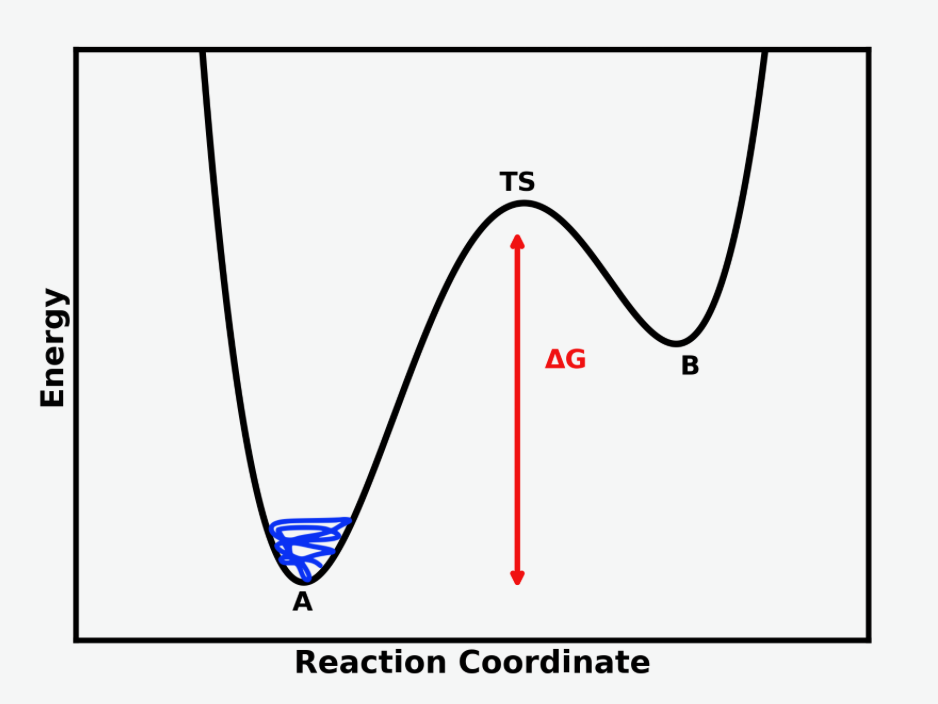
\includegraphics[width=0.6\textwidth]{images/motivation_img.png}
    \caption{Free Energy Barrier}%
    \label{fig:free_energy_barrier}%
\end{figure}

\section{Theory}

\subsection{Umbrella Sampling}
Consider some system with a potential $U(r^N)$. 
Traditional sampling methods may suffer from poor ergodicity due to certain energy landscapes, particularly if the confifuration space has many high-energy barriers that may trap the trajectory in a local minimum.
Introduced by Torrie and Valleau in 1977, umbrella sampling uses bias potentials to encourage sampling of potentially inaccessible states.
The biased distributions are then used to reconstruct an unbiased distribution and calculate quantities of interest, such as the free energy of the system.

\subsubsection{Reaction Coordinate}
We will introduce the notion of a reaction coordinate $q = f(r^N)$, an abstract typically one-dimensional parameter that unambiguously measures progress along a reaction pathway or transition between states.
Some examples of a reaction coordinate, both geometric and non-geometric, include bond distance, bond angle, torsion, dihedral angle, bond order, Hydrogen bonds, and RMSD. 
The free energy of a system is often considered as a function of reaction coordinate to demonstrate in some schematic form the potential energy profile associated to the reaction.

\subsubsection{Bias Potentials}
Umbrella sampling introduces a window-specific soft restraint biasing potential $W_k(q)$, such that the total potential for window $k$ becomes $U_k^\text{biased}(r^N) = U(r^N) + W_k(f(r^N))$.
Often, the restraint is chosen to be a harmonic potential of the form $W_k(f(r^N)) = \frac{1}{2} \kappa (f(r^N) - s_k)^2$ centered around a chosen $s_k$.
Some examples of bias functions added to a potential are shown below:

\begin{figure}[h]%
    \centering
    \subfloat[\centering Two-welled potential with selected bias functions]{{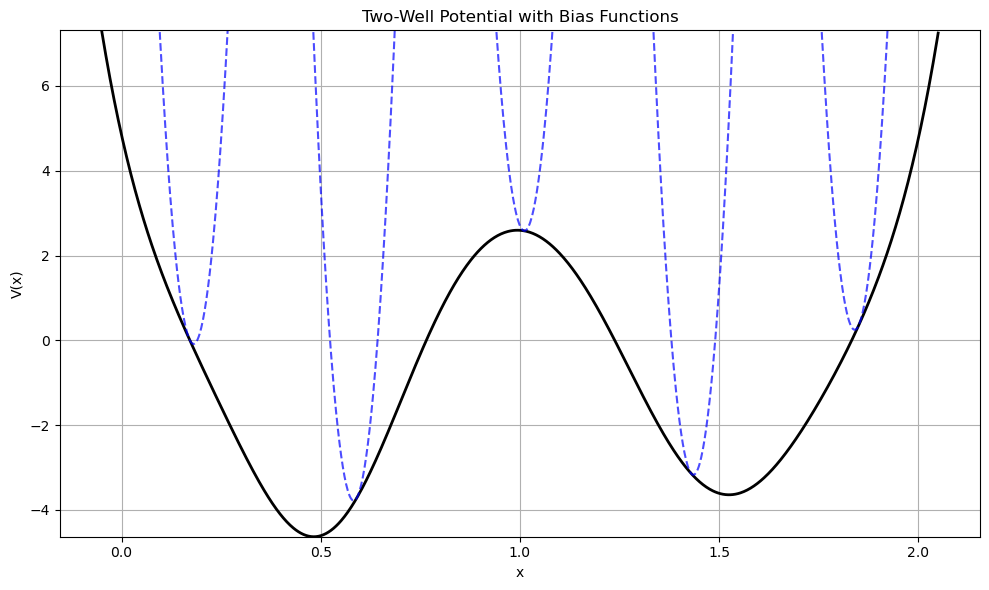
\includegraphics[width=0.46\textwidth]{images/two_well_with_bias.png} }}%
    \qquad
    \subfloat[\centering Two-welled potential with 100 bias functions]{{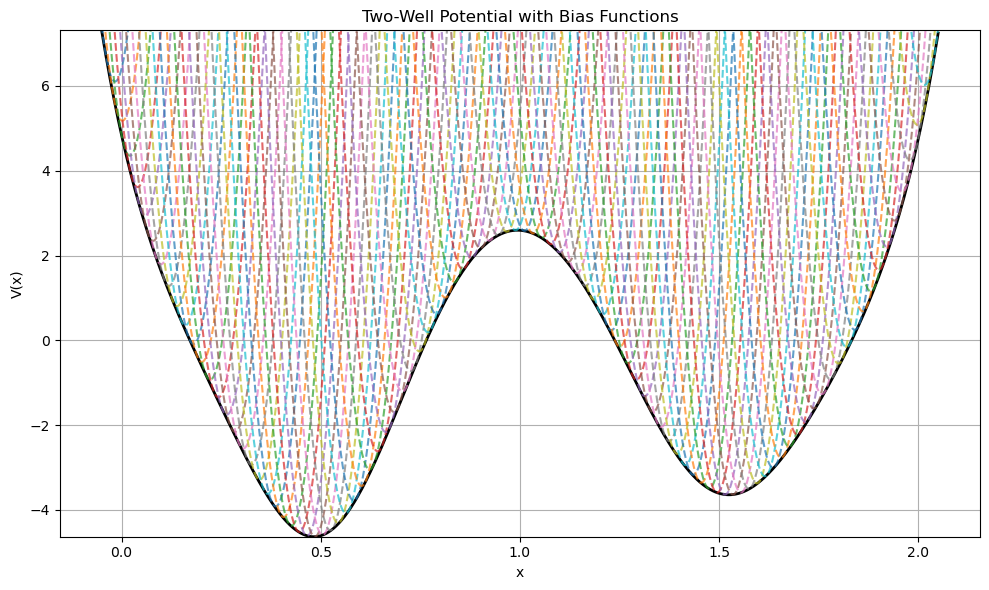
\includegraphics[width=0.46\textwidth]{images/two_well_all_bias.png} }}%
    \caption{Potentials with added bias}%
    \label{fig:bias_pots}%
\end{figure}

\subsubsection{Simulations}
In umbrella sampling, run a series of $n$ simulations with different biasing potentials, collecting a biased distribution of values of $q$.
Essentially, each simulation can be thought of as generating a histogram of values of $q$ primarily located within the "window" corresponding to the bias potential chosen.
The aim following the computation of these biased distributions is to first unbias them, and then to use the unbiased distributions to calculate the free energy of the system.
In figure \ref{fig:bias_pots}, this corresponds to running one simulation with each of the bias potentials shown in (b).

\subsection{WHAM}
The weighted histogram analysis method (WHAM) is the method for unbiasing the biased distributions that is used in conjunction with umbrella sampling.
We begin with biased probabilities $\tilde{P}_k(q)$ derived from the observed histograms from each biased simulation $k$.
Our goal is to construct an unbiased global probability distribution $P(q)$ over the reaction coordinate by unbiasing the individual biased distributions and stitching them together to minimize the expected statistical error.

\subsubsection{Unbiasing the Probabilities}
We aim to unbias the probability distributions $\tilde{P}_k(q)$, which can be done as follows:
$$ P_k(q) = e^{-\beta(A_k - A_0)} e^{\beta W_k(q)} \tilde{P}_k(q) $$
In this formulation, $A_k$ represents the free energy due to the $k$th bias potential and $A_0$ is an arbitrary parameter that stems from the fact we do not know the absolute free energies of any of our biased systems, only their relative free energies.
Recall that $W_k$ is the $k$th bias potential.
The first weighting term, $e^{-\beta(A_k - A_0)}$, corrects for the relative free energy shift introduced by each bias potential. It ensures that the biased distributions are properly scaled relative to each other, allowing them to be combined into a single, unbiased distribution.
The second weighting term, $e^{\beta W_k(q)}$, directly counteracts the effect of the bias potential, effectively unweighting the biased distribution. This makes intuitive sense as, for example, any observations where the bias potential was very high should be considered to be more significant as it is indicative that the underlying potential must favor that state.

% $$\tilde{P}(q, s_k) = e^{\beta A_k} \int d^N r^N e^{-\beta U(r^N)} e^{- \beta W(f(r^N), s^{(k)})}\delta(f(r^N) - q)$$
% We can then express the free energy due to each individual restraining potential, $A_k$, as follows:
% $$e^{-\beta A_k} = \int d^N r^N e^{-\beta U(r^N)} e^{-\beta W(f(r^N), s^{(k)})} = e^{-\beta A_0} \left \langle e^{- \beta W(f(r^N), s^{(k)})} \right \rangle$$
% Note the following:
% $$e^{-\beta A_0} = \int d^N r^N e^{-\beta U(r^N)} = Z$$
% We can use this process to calculate the unbiased potential from the $k$-th window as follows:
% $$ P_k(q) = e^{-\beta(A_k - A_0)} e^{\beta W\left(q, s^{(k)}\right)} \tilde{P}(q, s^{(k)}) $$

\subsubsection{Reconstructing the Global Distribution}
Our aim is to use the $k$ unbiased probability functions from the simulations to construct the global distribution $P(q)$ while minimizing statistical error.
We can set this up as follows:
\begin{align*}
    P(q) = &\sum_{k=1}^n C_k(q) P_k(q)\\
    \text{subject to} &\sum_{k=1}^n C_k(q) = 1
\end{align*}
The aim is to optimize the statistical error of $P(q)$ while satisfying the given constriant.
\\\\
The total statistical error in the global distribution will be:
$$ \sigma^2 = \sum_{k=1}^n C_k^2(q) \sigma_k^2 $$
Where $\sigma_k^2$ is the statistical error in the $k$th unbiased distribution.
Through error propagation, this can be related to the statistical error in the $k$th biased distribution, which in turn depends on the number of samples taken, the width of the intervals used for analyzing $q$, and the values of $\tilde{H}_k$.
\\\\
We can use Lagrange multipliers to perform this constrained minimization by instead minimizing the following:
$$ \Sigma^2 = \sum_{k=1}^n C_k^2(q) \sigma_k^2 - \lambda \left(\sum_{k=1}^n C_k(q) - 1\right)$$
After solving for $\lambda$ and $C_k(q)$ for all $k$ by setting $\frac{\partial \Sigma^2}{\partial C_k(q)} = 0$, we can plug the $C_k(q)$ coefficients back into the equation for $P(q)$, which provides us with a set of equations to solve iteratively for $P$ and $A_k$:
\begin{align*}
    P(q) &= \frac{\sum_{k=1}^n n_k \tilde{P_k}(q)}{\sum_{k=1}^n n_k e^{\beta (A_k - A_0)} e^{-\beta W_k(q)}}\\
    e^{-\beta (A_k - A_0)} &= \int \text{d}q \ P(q) e^{-\beta W_k(q)}
\end{align*}

Following the iterative solving of these equations, we can obtain the free energy from $P(q)$ through the following formula:
$$ A(q) = -\frac{1}{\beta} \ln P(q) + A_0 $$


\section{Systems}
In this project, we apply umbrella sampling and WHAM to three main systems: a one-dimensional two-welled potential, a one-dimensional multi-welled potential, and \textbf{a two-dimensional Muller-Brown potential}, which are shown in figure \ref{fig:system_pots}. These energy landscapes are chosen to demonstrate the effectiveness of umbrella sampling and WHAM when applied to systems with energy barriers that impede adequate sampling of configurational space in standard simulations. In all of these systems, we consider the only \textit{one} particle in the system, and the reaction coordinate is the position of this particle. Additionally, we consider the system to be in thermal equilibrium at a temperature of $T = 50K$, to demonstrate the effectiveness of the methods in sampling the potential energy surface at a low temperature.

\begin{figure}[h]%
    \centering
    \subfloat[\centering Two-Welled Potential]{{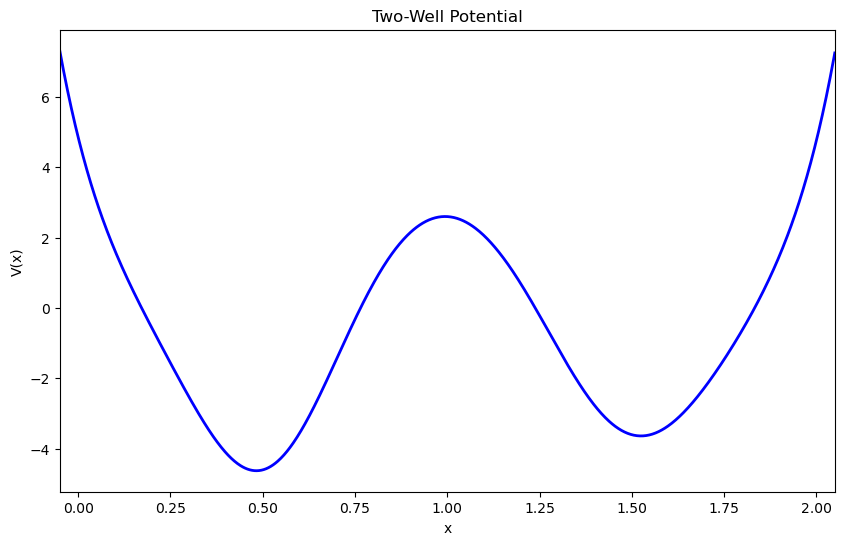
\includegraphics[width=0.46\textwidth]{images/two_well_V.png} }}%
    \qquad
    \subfloat[\centering Multi-Welled Potential]{{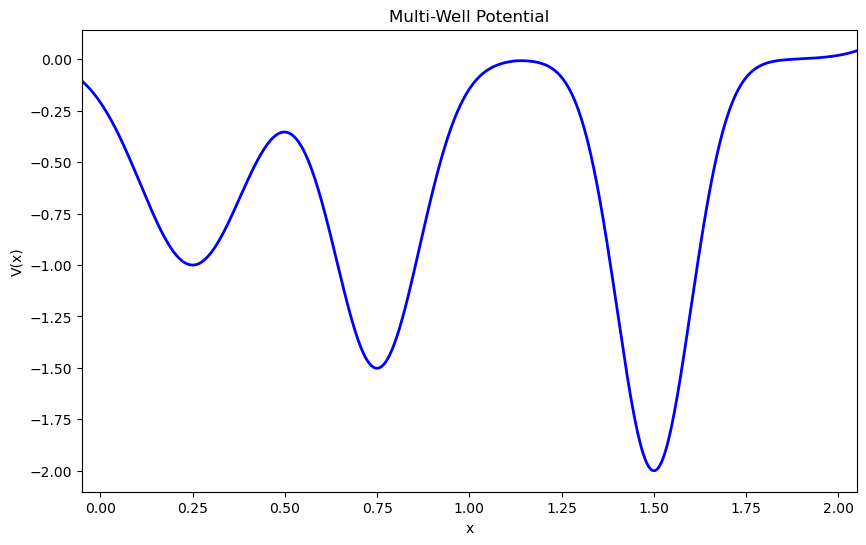
\includegraphics[width=0.46\textwidth]{images/multi_well_V.png} }}%
    \caption{Potentials Used}%
    \label{fig:system_pots}%
\end{figure}

\subsection{1D Two-Welled Potential}

We first consider a simple one-dimensional two-welled potential of the form:

$$
V(x) = 5(x-1)^8 - \epsilon_0 e^{-\frac{\epsilon_0(x-0.5)^2}{\sigma^2}} + \epsilon_1 e^{-\frac{\epsilon_1(x-1.0)^2}{\sigma^2}} - \epsilon_2 e^{-\frac{\epsilon_2(x-1.5)^2}{\sigma^2}}
$$

Where $\epsilon_0 = 5$, $\epsilon_1 = 3$, $\epsilon_2 = 4$, and $\sigma = 0.6$. 
This potential has two wells at $x = 0.5$ and $x = 1.5$, and a barrier at $x = 1.0$, as seen in Figure \ref{fig:system_pots}

\subsection{1D Multi-Welled Potential}

We then consider a one-dimensional multi-welled potential of the form:
\begin{align*}
    V(x) = 5 \min_{i} \left((x - x_i)^8\right) - \sum_  {i=1}^{3} \epsilon_i e^{-\frac{\epsilon_i(x-x_i)^2}{\sigma^2}}
\end{align*}
Where $x_1 = 0.25$, $x_2 = 0.75$, $x_3 = 1.5$, $\epsilon_0 = 1.0$, $\epsilon_1 = 1.5$, $\epsilon_2 = 2.0$, and $\sigma = 0.2$. This potential has three wells at $x = 0.25$, $x = 0.75$, and $x = 1.5$, as seen in Figure \ref{fig:system_pots}.

% \subsection{2D Muller-Brown Potential}

% Finally, we consider the two-dimensional Muller-Brown potential, which is a model potential energy surface that is often used to test optimization algorithms. The potential is given by:

% \begin{align*}
%     V(x, y) = \sum_{i=1}^{4} A_i e^{a_i(x - x_i)^2 + b_i(x - x_i)(y - y_i) + c_i(y - y_i)^2}
% \end{align*}

% Where $A_1 = -200$, $A_2 = -100$, $A_3 = -170$, $A_4 = 15$, $a_1 = -1$, $a_2 = -1$, $a_3 = -6.5$, $a_4 = 0.7$, $b_1 = 0$, $b_2 = 0$, $b_3 = 11$, $b_4 = 0.6$, $c_1 = -10$, $c_2 = -10$, $c_3 = -6.5$, $c_4 = 0.7$, $x_1 = 1$, $x_2 = 0$, $x_3 = -0.5$, $x_4 = -1$, $y_1 = 0$, $y_2 = 0.5$, $y_3 = 1.5$, $y_4 = 1$.

% \begin{figure}%
%     \centering
%     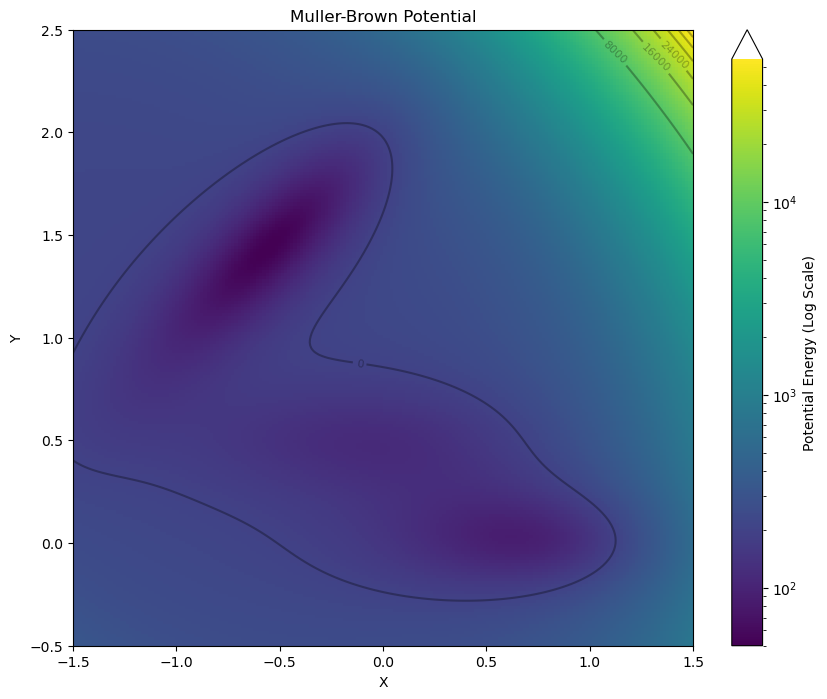
\includegraphics[width=0.6\textwidth]{images/muller_brown_V.png}
%     \caption{2D Potential}%
%     \label{fig:2D_pot}%
% \end{figure}

% This potential has three minima and two saddle points, as seen in Figure \ref{fig:2D_pot}, and is often used for testinmg algorithms that explore transition states and barriers. 

\section{Results}

\subsection{1D Two-Welled Potential}

We divided our one-dimensional two-welled potential into 100 windows, each with a biasing potential of the form $W_k(x) = \frac{1}{2} \kappa (x - s_k)^2$ with $\kappa = 2000$, where $s_k$ is the center of the $k$th window, evenly spaced out across the range of $x$. We then ran MCMC simulations in each window, obtaining 100,000 samples for each window, resulting in biased distributions of $x$.

\subsubsection{Sampling}
% \begin{figure}%
%     \centering
%     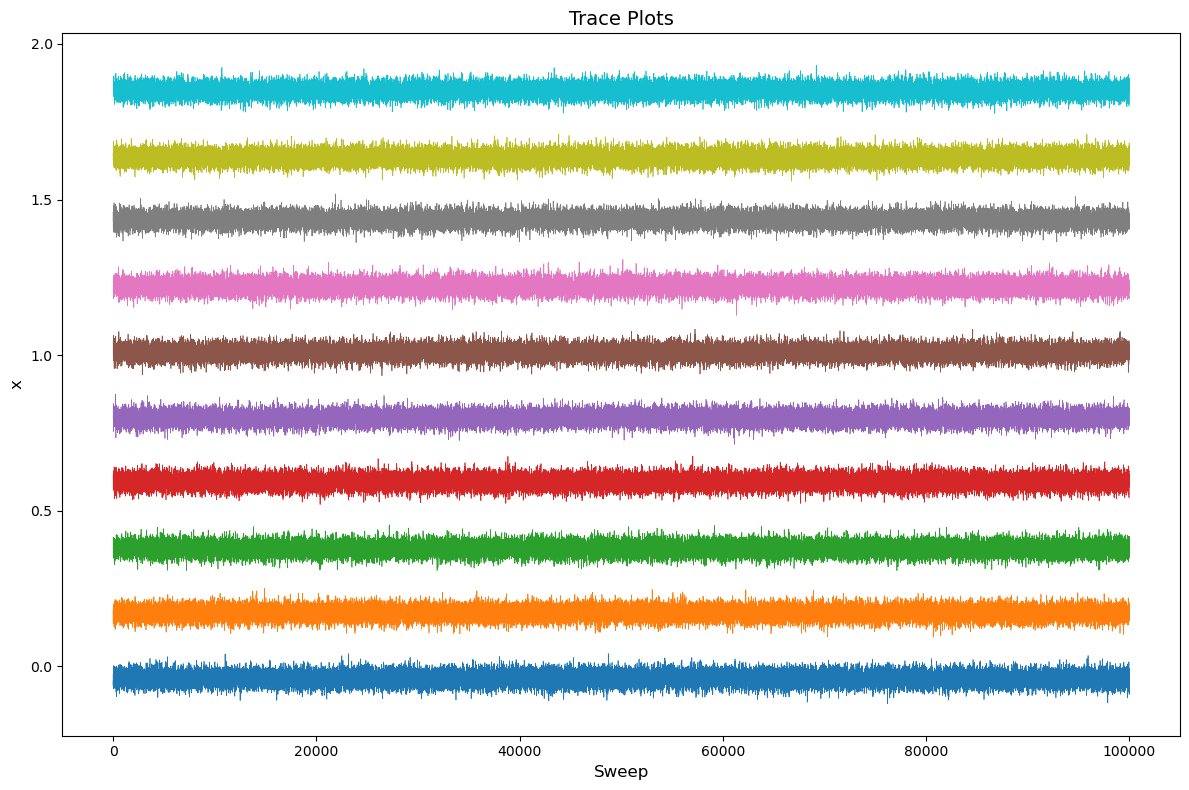
\includegraphics[width=0.6\textwidth]{images/two_well_V_trace_plot.png}
%     \caption{Trace Plot}%
%     \label{fig:trace_plot_two_well}%
% \end{figure}

\begin{figure}[h]%
    \centering
    \subfloat[\centering Trace Plot]{{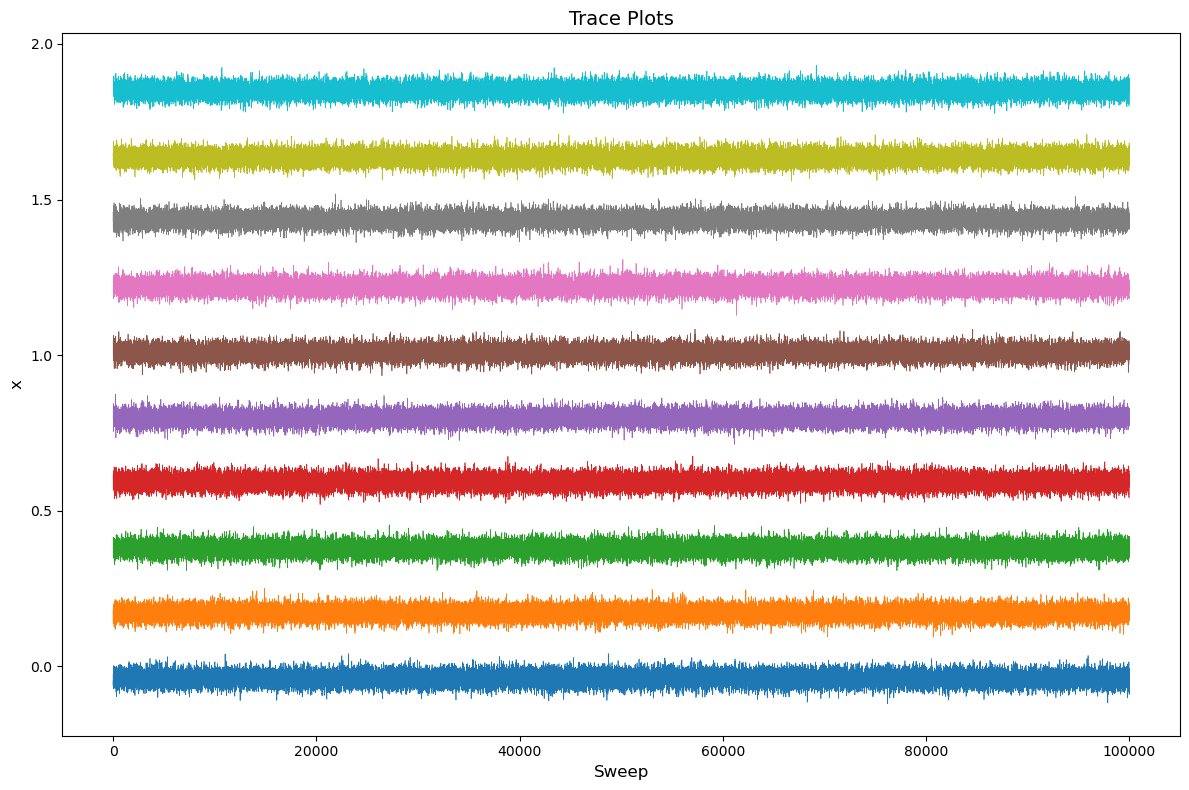
\includegraphics[width=0.46\textwidth]{images/two_well_V_trace_plot.png} }}%
    \qquad
    \subfloat[\centering Sampled Densities]{{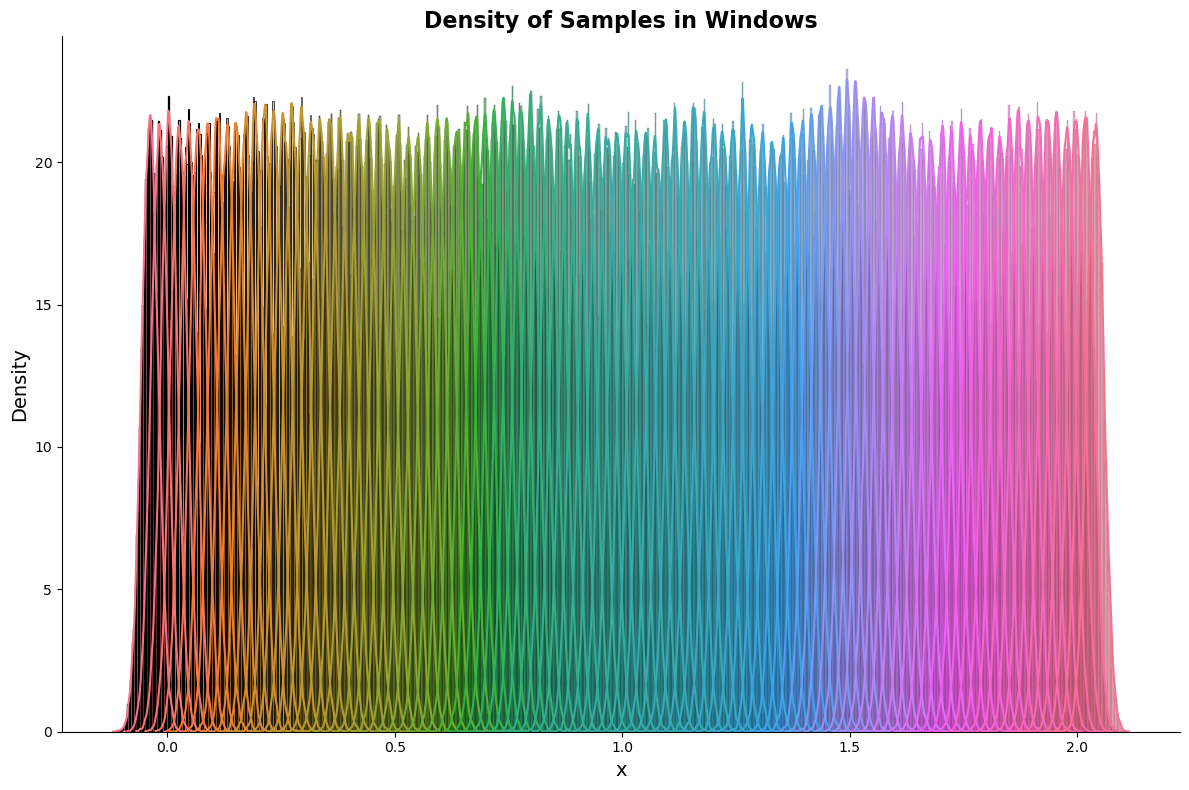
\includegraphics[width=0.46\textwidth]{images/two_well_window_sample_dens.png} }}%
    \caption{Confirmation of Window Sampling Success}%
    \label{fig:converge_diag}%
\end{figure}

In Figure \ref{fig:converge_diag}, we plot the trace plot of the biased distributions of $x$ for 10 windows. We can see that the samples are stable and oscillate around the center of the window, indicating that the biasing potential has effectively encouraged sampling in the regions of the potential that would otherwise be difficult to sample. This gives us confirmation that the biasing potential is working as intended.
\\\\
Additionally, we plot the sampled densities of $x$ for all the windows in Figure \ref{fig:converge_diag}. We can see that the sampling results in a relatively flat distribution, indicating that the biasing potential has effectively encouraged sampling in the regions of the potential that would otherwise be difficult to sample. In addition, the sampled densities overlap, indicating that our choice of $\kappa$, the biasing spring constant, was appropriate given our number of windows, and our computed free energy profile should be accurate and continuous.

\subsubsection{Unbiasing and Free Energy Profile}

\begin{figure}[h]%
    \centering
    \subfloat[\centering Unbiased Probabilities]{{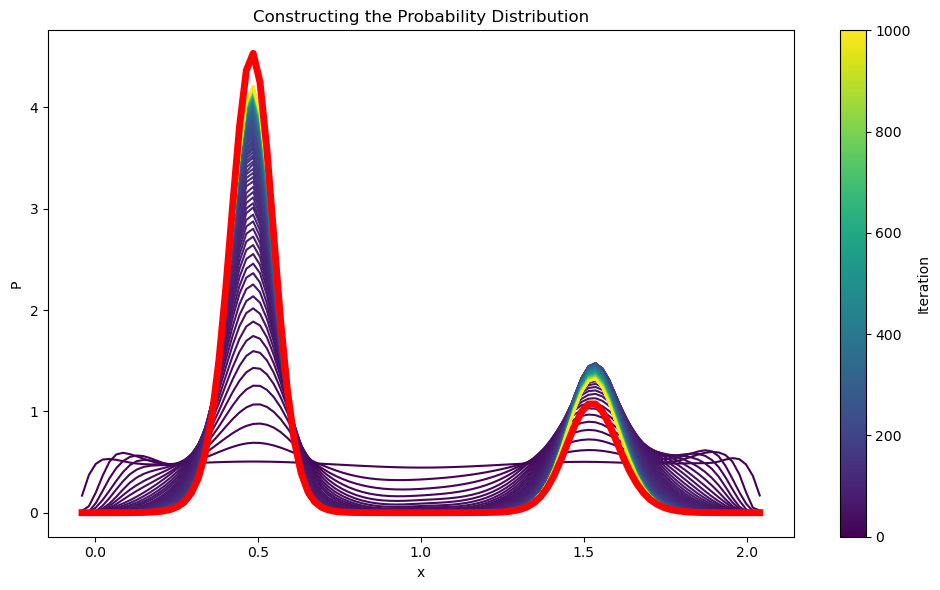
\includegraphics[width=0.45\textwidth]{images/two_well_wham.png} }}%
    \qquad
    \subfloat[\centering Free Energy Profile]{{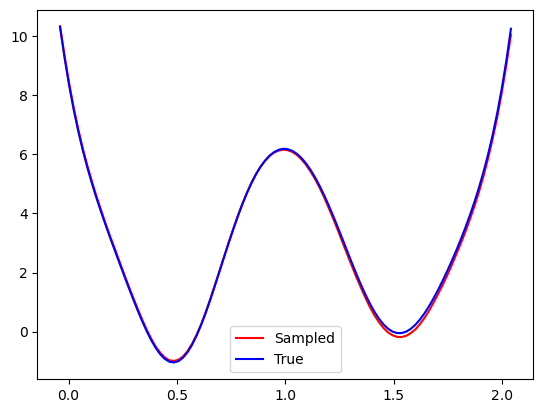
\includegraphics[width=0.47\textwidth]{images/two_well_free_energy.png} }}%
    \caption{Unbiased Densities and Free Energy Profile}%
    \label{fig:unbiased_densities}%
\end{figure}

Next, we applied WHAM to unbias the biased distributions and reconstruct the global probability distribution across $x$. We then calculated the free energy profile of the system.

In Figure \ref{fig:unbiased_densities}, we plot the global unbiased probabilities of $x$ for every iteration of WHAM. We can see that the probabilities converge to a stable distribution, closely approximating the true distribution of $x$ in the system (the red curve), which is given by $P(x) \propto e^{-\beta V(x)}$. This indicates that WHAM has successfully unbiased the biased distributions. Similarly, we see that the computed free energy profile of the system as a function of $x$ is accurate.

\subsubsection{Comparison with Metropolis-Hastings}

We also compared the energy profile obtained from umbrella sampling and WHAM with the energy profile obtained from a standard Metropolis-Hastings simulation. We ran a Metropolis-Hastings simulation for 1,000,000 steps, and calculated the free energy profile of the system as a function of $x$.

\begin{figure}[h]%
    \centering
    \subfloat[\centering Probability Distribution]{{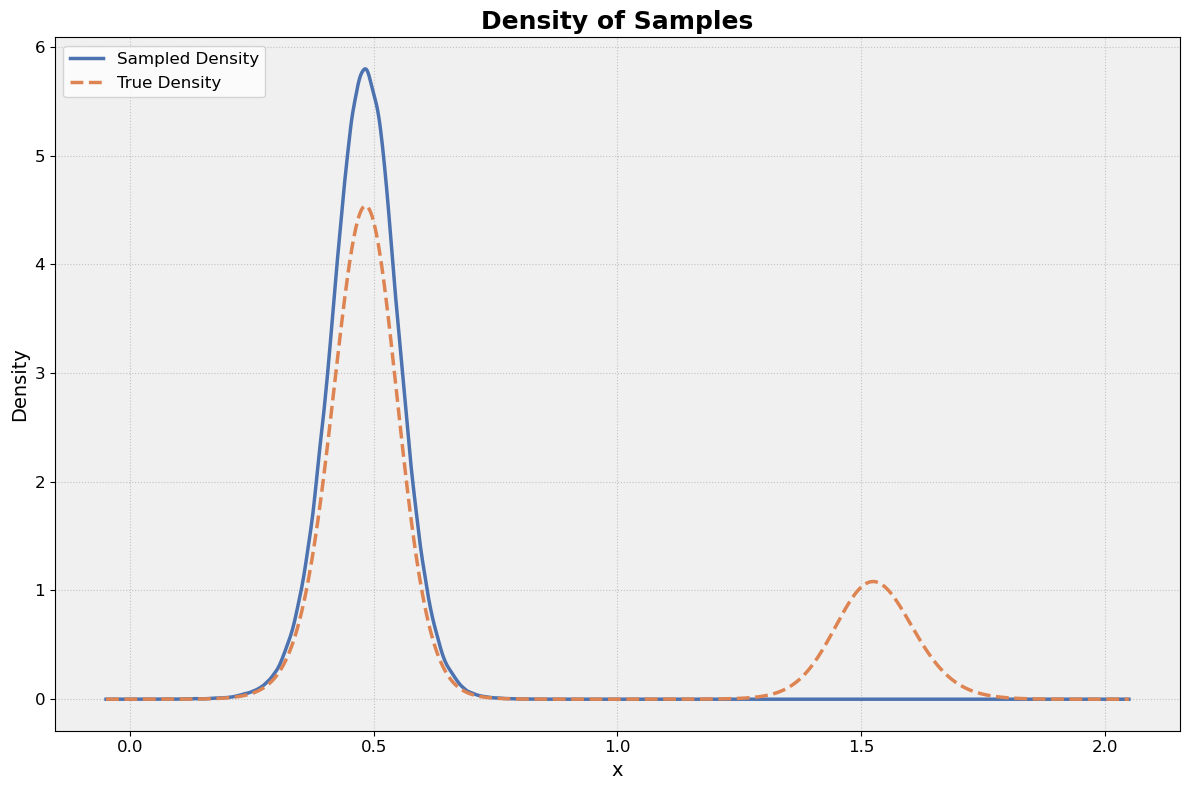
\includegraphics[width=0.46\textwidth]{images/metro_hastings_density.png} }}%
    \qquad
    \subfloat[\centering Free Energy Profile]{{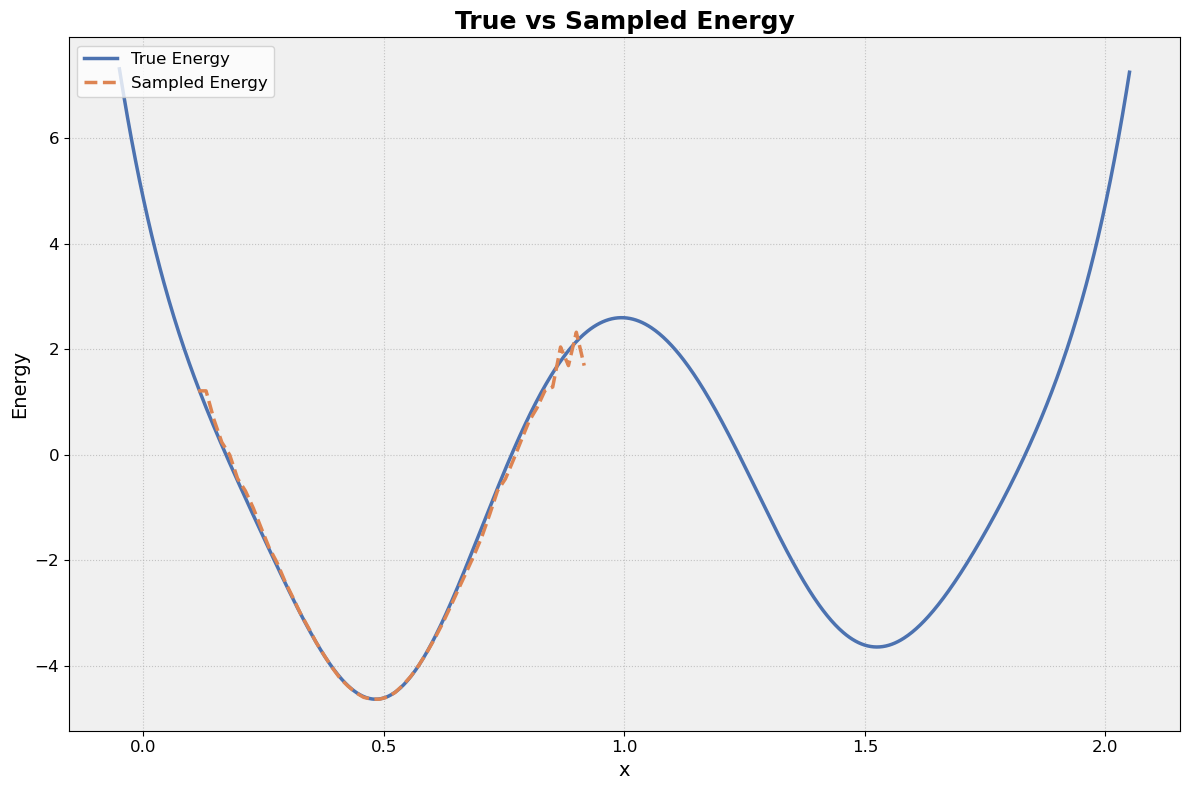
\includegraphics[width=0.46\textwidth]{images/metro_hastings_energy.png} }}%
    \caption{Metropolis-Hastings Simulation Results}%
    \label{fig:metro_hastings_plot}%
\end{figure}

In Figure \ref{fig:metro_hastings_plot}, we plot the probability distribution across $x$ obtained from the Metropolis-Hastings simulation and the potential energy profile of the system. We can see that because of the high energy barrier in the potential, as well as the low temperature of the system, the standard Metropolis-Hastings simulation is unable to sample the potential energy surface effectively, and gets stuck in the local minima. This results in a free energy profile doesn't fully capture the entire domain of the system. In contrast, the free energy profile obtained from umbrella sampling and WHAM captures the entire domain of the system, and is able to accurately sample the potential energy surface.

\subsection{1D Multi-Welled Potential}

Similarly, we divided our one-dimensional multi-welled potential into 100 windows, each with a biasing potential of the same form as the two-welled potential. We then ran MCMC simulations in each window, obtaining $100,000$ samples for each window, resulting in biased distributions of $x$. We show the evolution of the global unbiased probability distribution and the reconstructed free energy profile from the umbrella sampling below:

\begin{figure}[h]%
    \centering
    \subfloat[\centering Unbiased Probabilities]{{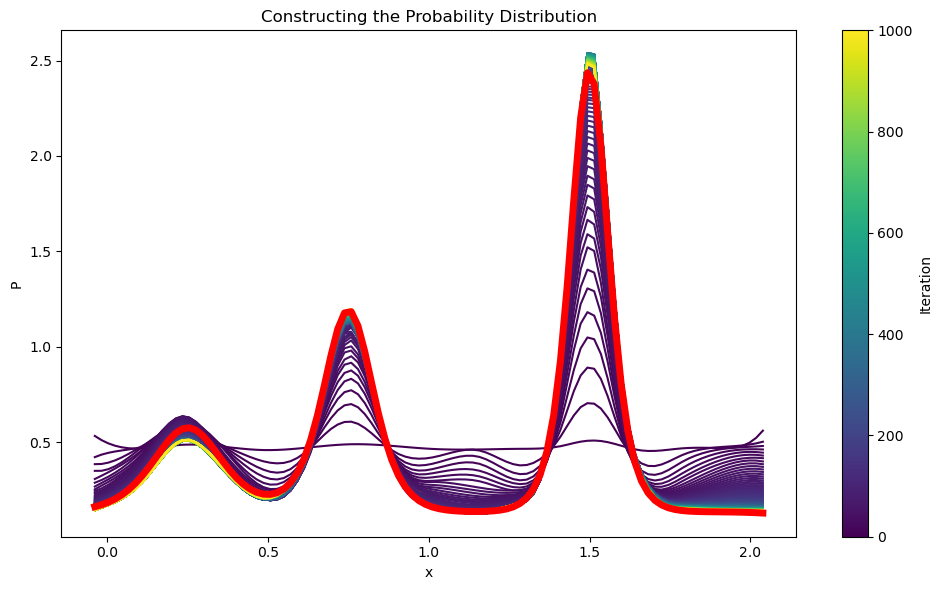
\includegraphics[width=0.45\textwidth]{images/multi_well_wham.png} }}%
    \qquad
    \subfloat[\centering Free Energy Profile]{{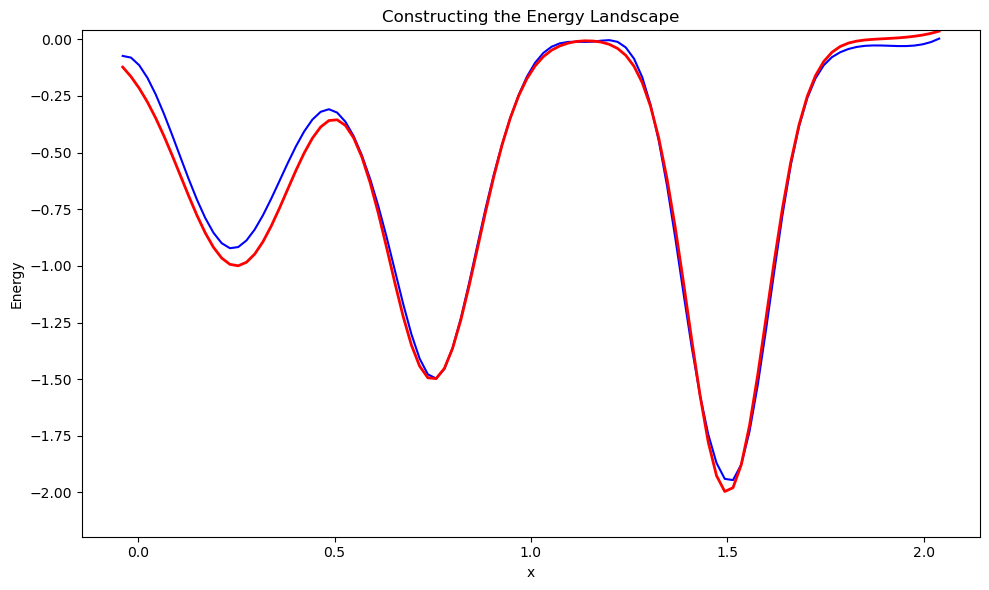
\includegraphics[width=0.47\textwidth]{images/multi_well_free_energy.png} }}%
    \caption{Unbiased Densities and Free Energy Profile}%
    \label{fig:unbiased_densities}%
\end{figure}
As we can see from these plots, our method generalizes well to more complex potential functions, accurately reconstructing the expected probability distribution and the true free energy profile. 

\section{Next Steps}


\begin{thebibliography}{9}

\bibitem{ferguson}
Andrew Ferguson (2025), \emph{MENG 25500, Classical Molecular and Materials Modeling}

\bibitem{youtube}
MoBioChem (2020), \emph{Enhanced Sampling Methods - Chapter 2: Umbrella Sampling}

\bibitem{textbook}
Johannes Kastner (2011), \emph{Umbrella sampling}

\end{thebibliography}

\end{document}
